\chapter{Metriche}\label{ch:chapter1}

Le protagoniste della nostra analisi sono, come anticipato nell'introduzione: 
\textbf{Improved Precision and Recall}, \textbf{Density and Coverage}, \textbf{Probabilistic Precision and Recall} e \textbf{Precision and Recall Coverage}. 
Saranno poi introdotte tecniche più recenti come la \textbf{Precision Recall Curve} e altre metriche correlate.\

Tutte le metriche citate hanno una serie di caratteristiche in comune, il primo, e forse più ovvio, è che sono presentate in coppia. 
Questo perchè queste coppie di metriche cercano misurare due aspetti complementari delle reti generative: la \textbf{Fidelity} e la \textbf{Diversity}.\ 

Il secondo aspetto che hanno in comune, che verrà discusso e approfondito invece nelle sezioni seguenti, è relativo a come queste metriche sono misurate. Ciascuna di esse infatti 
si basa su un calcolo simile dipendente dalla distanza tra campioni generati e reali e la distanza \textbf{interset} vale a dire fra campioni vicini di uno stesso insieme.\

È utile definire meglio i concetti appena accennati: 
\begin{itemize}
    \item \textbf{Fidelity}: è la somiglianza tra i campioni generati e quelli reali.
    \item \textbf{Diversity}: è la varietà tra i campioni generati.
    \item \textbf{Precision}: misura la proporzione di campioni generati che ricadono nel supporto della distribuzione reale.
    \item \textbf{Recall}: misura la proporzione di campioni reali che ricadono nel supporto della distribuzione generata.
\end{itemize}

\begin{figure}[htbp]
    \centering
    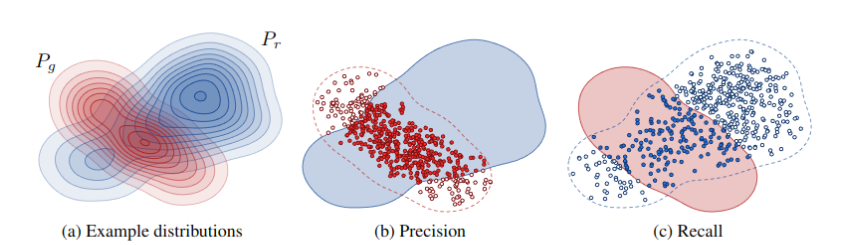
\includegraphics[width=\linewidth]{../images/2_PrecisionRecallManifold_si.png}
    %\label{fig:precision-recall-manifold}
    %\source{\cite{2ImprovedPrecisionRecall} Figure 1}
\end{figure}

Sebbene \textit{fidelity} e \textit{diversity} siano concetti centrali per la valutazione della qualità dei modelli generativi, risultano difficili da quantificare direttamente a causa della loro natura astratta.
Si riduce quindi il problema del calcolo della \textit{fidelity} e \textit{diversity} a quello della \textit{precision} e \textit{recall} (che offrono una formalizzazione più operativa di questi concetti, fornendo una base matematica per una valutazione quantitativa).\

Entrambe si basano sul concetto di \textbf{supporto} della distribuzione. Dato un numero limitato di campioni, definire un supporto continuo è un problema non banale. 
Molte delle metriche si preoccupano quindi di stimare il supporto e stabilire un criterio operativo per determinare la somiglianza tra due distribuzioni, il grado di sovrapposizione dei supporti stimati.
In questo contesto la stima del supporto è detta \textbf{manifold}.

\section{Improved Precision and Recall}
\label{sec:improved-precision-and-recall}

Nonostante il nome \textit{Improved Precision and Recall} possa suggerire un miglioramento rispetto a una versione precedente e meno sofisticata di \textit{precision and recall}, 
la metrica proposta da Tuomas Kynkäänniemi et al., 2019 \cite{2ImprovedPrecisionRecall}, precede temporalmente, in realtà, quella che sarà presentata successivamente, ovvero la metrica denominata più semplicemente \textit{Precision and Recall Coverage}. 
Di fatto, si tratta della forma più semplice di \textit{precision-recall} analizzata in questo lavoro, e rappresenta il punto di partenza per la nostra analisi.

Sia \(R\) il dataset di campioni reali (in genere dati usati per l'addestramento della rete) e \(G\) il dataset di campioni generati dalla rete neurale, identifichiamo con \boldsymbol{\Phi_R} e \boldsymbol{\Phi_G} (tendenzialmente con \boldsymbol{\Phi_R} = \boldsymbol{\Phi_G}) lo spazio delle caratteristiche e \(\Phi_R\) e \(\Phi_G\) i vettori di feature estratti da \(R\) e \(G\) rispettivamente.

È importante sottolineare che, come vedremo anche successivamente nella parte sperimentale, la scelta dell'estrattore di feature è cruciale per la corretta valutazione delle metriche di valutazione dei GAN.

Il manifold stimato a partire da \(R\) e \(G\) è un insieme di ipersfere, ciascuna con un raggio definito e centrate nei vari punti di \(\Phi_R\) e \(\Phi_G\). Il raggio di queste ipersfere è 
determinato da un iperparametro \texttt{k} che rappresenta il numero dei \textbf{nearest neighbors (NN)} da considerare. 

Possiamo quindi definire una funzione binaria che determini se un certo punto appartiene al manifold o meno:
\begin{equation}
    f_{ipr}(x, \Phi) = 
    \begin{cases}
        1 & \text{if }~~ \exists ~ y \in \Phi \text{ such that } ||x - y||_2 \leq ||y - NN_k(y, \Phi)||_2 \\
        0 & \text{otherwise.}
    \end{cases}
\end{equation}

Dove \(NN_k(y, \Phi)\) è il \texttt{k}-esimo vicino più prossimo di \texttt{y} in \(\Phi\).

La Precision e la Recall possono essere quindi definite come:
\begin{equation}
    Precision(\Phi_R, \Phi_G) = \frac{1}{|\Phi_G|} \sum_{g \in \Phi_G} f_{ipr}(g, \Phi_R)
\end{equation}
\begin{equation}
    Recall(\Phi_R, \Phi_G) = \frac{1}{|\Phi_R|} \sum_{r \in \Phi_R} f_{ipr}(r, \Phi_G)
\end{equation}

Nominalmente la Precision misura la percentuale di punti di \(\Phi_G\) che ricadono nel manifold di \(\Phi_R\) e la Recall la percentuale dei punti di \(\Phi_R\) che ricadono nel manifold di \(\Phi_G\).
Come tali le due metriche sono quindi normalizzate e assumono valori compresi tra \texttt{0} e \texttt{1}.
Come ripeteremo in seguito la metrica risulta dipendente dall'iperparametro \texttt{k} e in particolare pare che per \texttt{k = 3} si ottengano i risultati migliori.

\section{Density and Coverage}
\label{sec:density-and-coverage}

Come vedremo nel capitolo seguente l'\textit{Improved Precision Recall} soffre la presenza di \textit{outliers} nei datasets, vale a dire che il manifold stimato da \(R\) e \(G\) può essere fortemente influenzato da pochi punti molto distanti dalla distribuzione principale e quindi la presenza di molti dati generati in una zona vicina a questi outliers può portare a un errata alta stima della \textit{fidelity-precision}.
La \textit{Density and Coverage} è una metrica che cerca di mitigare questo problema (come analizzato da Muhammad Ferjad Naeem et al., 2019 \cite{3ReliableFidelityDiversityMetrics}). 

Invece che contare se le varie ipersfere in $\Phi_R$ contengono almeno un punto di $\Phi_G$, la \textit{Density} conta quanti punti di $\Phi_G$ sono inclusi in ciascuna ipersfera centrata su $\Phi_R$. Viene quindi scalato il risultato per il numero di ipersfere totali per il valore di \texttt{k} (si suppone che ciascuna ipersfera contenga almeno \texttt{k} punti).
Questo conporta però che la \textit{density} non è una metrica normalizzata e in certi casi assume valori maggiori di \texttt{1}. La formula è la seguente: 
\begin{equation}
    Density(\Phi_R, \Phi_G) = \frac{1}{k|\Phi_G|} \sum_{g \in \Phi_G} \sum_{r \in \Phi_R} \mathbbm{1}_{||r - g||_2 \leq ||g - NN_k(g, \Phi_G)||_2}
\end{equation}

Rispetto alle altre metriche in cui si poteva apprezzare la simmetria fra le formule per la stima di \textit{fidelity} e \textit{diversity}, in questo caso la \textit{Coverage} è una metrica completamente diversa dalla \textit{Density}. Questo perchè rispetto a $\Phi_G$, $\Phi_R$ non dovrebbe presentare \textit{outliers}.
La Coverage valuta se ogni dato reale \(r \in \Phi_R \)​ è rappresentato da almeno un punto generato \(g \in \Phi_G \)​, costruendo il manifold in \(\Phi_R\) e verificando se esiste almeno un punto di \(\Phi_G\) in ciascuna ipersfera. 

Anticipando la sezione che seguirà \textit{Precision Recall Curve}, è utile definire una funzione binaria che determini per la \textit{Coverage} se un certo punto appartiene a questa nuova definzione di manifold:
\begin{equation}
    f_{cov}(x, \Phi_x, \Phi_y) = 
    \begin{cases}
        1 & \text{if }~~ \exists ~ y \in \Phi_y \text{ such that } ||x - y||_2 \leq ||x - NN_k(x, \Phi_x)||_2 \\
        0 & \text{otherwise.}
    \end{cases}
\end{equation}

La formula della metrica sarà quindi:
\begin{equation}
    Coverage(\Phi_R, \Phi_G) = \frac{1}{|\Phi_R|} \sum_{r \in \Phi_R} f_{cov}(r, \Phi_R, \Phi_G)
\end{equation}

La formula potrebbe sembrare molto simile a quella dell'Improved Precision ma con un'importante differenza, ci chiediamo se esiste almeno un punto di $\Phi_G$ per ciascuna ipersfera costruita su $\Phi_R$ e non se per ciascun punto di $\Phi_G$ esiste una ipersfera che lo contiene. 

\begin{figure}[htbp]
    \centering
    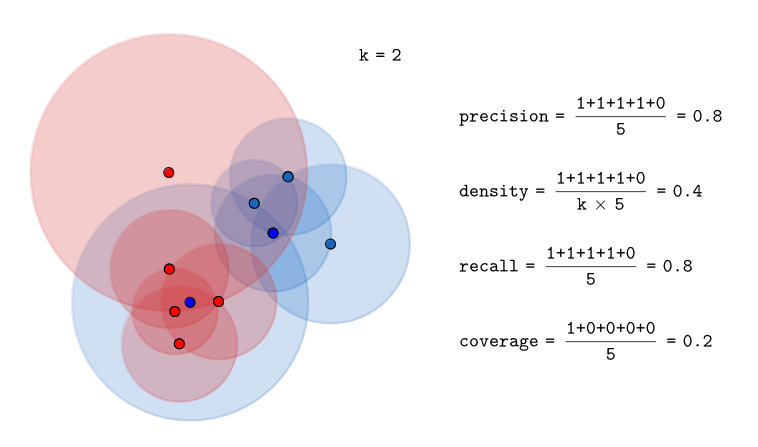
\includegraphics[width=\linewidth]{../images/prdc.png}
    %\label{fig:precision-recall-manifold}
    %\source{\cite{2ImprovedPrecisionRecall} Figure 1}
\end{figure}

Al contrario della Density, la Coverage è una metrica normalizzata e assume valori compresi tra 0 e 1.

Sperimentalmente, si è verificato che un valore di \texttt{k = 5} fornisce risultati ottimali, bilanciando la granularità delle ipersfere e la loro rappresentatività del manifold.

\section{Probabilistic Precision and Recall}  
\label{sec:probabilistic-precision-and-recall}

Un altro approccio al problema della stima del manifold consiste nel considerare la densità di probabilità delle distribuzioni reali e generate. Le formule utilizzate sono simili a quelle dell'\textit{Improved Precision e Recall},
ma con una differenza cruciale: invece di utilizzare una funzione di scoring binaria (\(f_{ipr}\)), si valuta la probabilità che un punto appartenga al manifold stimato. 
Questa probabilità viene calcolata dividendo il supporto in sottosupporti locali (\textit{subSupports}). 
Seguendo il lavoro di Dogyun Park et al., 2023 \cite{4ProbabilisticPrecisionRecall}, la probabilità di un punto \(x\) di appartenere a un sottosupporto centrato su \(y\) è definita come:
\begin{equation}
    P(x \in subSupp(y)) = 
    \begin{cases}
        1 - \frac{||x - y||_2}{\tau} & \text{se } ||x - y||_2 \leq \rho \\
        0 & \text{altrimenti.}
    \end{cases}
\end{equation}

La probabilità che un punto appartenga al manifold stimato viene quindi calcolata calcolando la probabilità che il dato non appartenga all'intersezione fra tutti i complementari dei sottosupporti locali
(supponendo quindi l'indipendenza degli eventi \(x \in subSupp^C(y)\) \(\forall y\)):
\begin{equation}
    P(x \in manifold(\Phi_y))) = 1 - \prod_{y \in \Phi_y} (1 - P(x \in subSupp(y)))
\end{equation}

Per la precision, la somma itera \(x\) su \(\Phi_G\) con manifold calcolato su \(\Phi_R\), mentre per la recall, si inverte il ruolo dei due dataset:
\begin{equation}
    Precision(\Phi_R, \Phi_G) = \frac{1}{|\Phi_G|} \sum_{g \in \Phi_G} P(g \in manifold(\Phi_R)),
\end{equation}
\begin{equation}
    Recall(\Phi_R, \Phi_G) = \frac{1}{|\Phi_R|} \sum_{r \in \Phi_R} P(r \in manifold(\Phi_G)).
\end{equation}

La variabile \(\rho\) gioca un ruolo cruciale in questo approccio, rappresentando il raggio delle ipersfere usate per stimare i sottosupporti locali. Per evitare sovrastime, si adotta una strategia simile alla \textit{Kernel Density Estimation} con varianza fissata, definendo \(\rho\) come segue:  
\begin{equation}
    \rho(\Phi) = \alpha \cdot \frac{1}{|\Phi|} \sum_{x \in \Phi} ||x - NN_k(x, \Phi)||_2
\end{equation}

dove \(\alpha\) è un nuovo iperparametro (con valore consigliato \(\alpha = 1.2\)). Per la precision si adotta quindi \(\rho(\Phi_R)\), mentre per la recall si utilizza \(\rho(\Phi_G)\).

L'approccio probabilistico è particolarmente utile perché affronta i limiti delle metriche basate sul \texttt{k}-Nearest Neighbor. La scelta di una \(\rho\) costante pari alla media delle distanze \(k\)-NN sopprime l’influenza degli outliers, riducendo la sovrastima del manifold in regioni scarsamente popolate 
e rende la metrica più robusta alla scelta di \texttt{k}, minimizzando la sensibilità della metrica ai cambiamenti del numero di vicini considerati.  

Sempre seguendo la letteratura il valore di \texttt{k} consigliato è \texttt{k = 4}.

\section{Precision and Recall Coverage}
\label{sec:precision-and-recall-coverage}

L'ultima metrica che verrà presentata è la \textit{Precision and Recall Coverage}, proposta da Fasil Cheema et al., 2023 \cite{1PrecisionRecallCover}.

Mantenendo la formalizzazione della sezione precedente si introduce un nuovo iperparametro \texttt{k' = Ck}. L'idea è quella di fornire un nuovo elemento per regolare la dimensione del manifold, e in particolare
le aree da considerare trascurabilmente piccole e quelle sufficientemente grandi. L'algoritmo proposto prevede per la Precision di costruire un manifold su \(\Phi_G\) con ipersfere con raggio pari alla distanza dal \texttt{k'}-th nearest neighbor
e contare il numero di ipersfere che contengono almeno \texttt{k} punti di \(\Phi_R\), si divide quindi per il numero di ipersfere totali (la dimensione di \(\Phi_G\)). 
Per la Recall si procede in modo analogo ma invertendo i ruoli di \(\Phi_R\) e \(\Phi_G\).

È importante notare come la metrica sia fondamentalmente la stessa della Coverage ma non è più sufficiente che esista un unico punto di \(\Phi_R\) in un ipersfera di \(\Phi_G\) ma è necessario invece che ce ne siano almeno \texttt{k}.
\begin{equation}
    Precision(\Phi_R, \Phi_G) = \frac{1}{|\Phi_G|} \sum_{g \in \Phi_G} \mathbbm{1}_{|\{ r \in \Phi_R, \text{s.t.} ||r - g||_2 \leq ||r - NN_{k'}(r, \Phi_R)||_2 \}| \geq k}
\end{equation}
\begin{equation}
    Recall(\Phi_R, \Phi_G) = \frac{1}{|\Phi_R|} \sum_{r \in \Phi_R} \mathbbm{1}_{|\{ g \in \Phi_G, \text{s.t.} ||g - r||_2 \leq ||g - NN_{k'}(g, \Phi_G)||_2 \}| \geq k}
\end{equation}

In questo caso l'aggiunta di un nuovo parametro, nonostante aumenti la complessità combinatoria di possibili valori assegnabili, si verifica sperimentalmente che mantenendo \texttt{C=3} la scelta di \texttt{k} e conseguentemente di \texttt{k'} può essere arbitraria
ottenendo comunque buoni risultati.

\section{Precision Recall Curve}  
\label{sec:precision-recall-curve}

Studi recenti \cite{5RevisitingPrecisionRecall, 6UnifyingPrecisionRecall, 7AssessingWithPrecisionRecall} hanno dimostrato che precision e recall possono essere interpretate come combinazioni lineari degli errori di tipo I e II di un classificatore binario ottimo.
Questa formulazione consente di costruire un limite superiore per la Precision e la Recall anche utilizzando un classificatore binario sub-ottimale. 
Inoltre, permette di analizzare il trade-off tra Precision e Recall tramite una curva, di cui le metriche viste in precedenza rappresentano solo i valori estremi.

I classificatori per la costruzione della curva Precision-Recall si basano sui manifold stimati. Le formule per i classificatori associati alle metriche sono:
\begin{equation}
    f_{\lambda}^{ipr}(x) = \mathbbm{1}_{\lambda \cdot |\{ r \in \Phi_R, \text{s.t.} ||r - x||_2 \leq ||r - NN_k(r, \Phi_R)||_2 \}| \geq |\{ g \in \Phi_G, \text{s.t.} ||g - x||_2 \leq ||g - NN_k(g, \Phi_G)||_2 \}|}
\end{equation}
\begin{equation}
    f_{\lambda}^{cov}(x) = \mathbbm{1}_{\lambda \cdot |\{ r \in \Phi_R, \text{s.t.} ||r - x||_2 \leq ||r - NN_k(x, \Phi_G)||_2 \}| \geq |\{ g \in \Phi_G, \text{s.t.} ||g - x||_2 \leq ||g - NN_k(x, \Phi_R)||_2 \}|}
\end{equation}

È interessante notare come le condizioni di appartenenza agli insiemi la cui cardinalità viene confrontata siano analoghe alle condizioni per \(f_{ipr}\) e \(f_{cov}\) con la differenza che qui andiamo a contare il numero di punti che soddisfano la condizione e non se esiste almeno un punto che la soddisfi.

La formula per \(f_{\lambda}^{ipr}\) può essere interpretata come una forma di Kernel Density Estimation (KDE) con bandwidth variabile.

\begin{equation}
    f_{\lambda}^{ipr}(x) = \mathbbm{1}_{\frac{\hat{p}(x)}{\hat{q}(x)} \geq \frac{1}{\lambda}},
\end{equation}

dove \(\hat{p}(x)\) e \(\hat{q}(x)\) rappresentano le densità stimate dai manifold reali e generati rispettivamente. In questa formulazione, il parametro \(\lambda\) agisce come un fattore di soglia che modula la decisione del classificatore:  

- \(\lambda \to 0\): Include quasi tutti i punti, abbassando la precisione e massimizzando la recall.  

- \(\lambda \to \infty\): Include solo i punti con densità generata molto bassa, massimizzando la precisione ma riducendo la recall.

Dal momento che questi classificatori vanno a cotruire un limite superiore, è possibile prendere il minimo fra le curve ottenute con i diversi classificatori per ottenere una stima più precisa.

\section{Altre metriche e funzioni correlate}
\label{sec:altre-metriche}

Per aggiungere un'appendice alla sezione precedente, sono state brevemente sfruttate altre metriche/classificatori accennati nel medesimi paper e in particolare nell'articolo di Benjamin Sykes et al, 2024 \cite{6UnifyingPrecisionRecall}. 
Tra questi risulta il knn classifier e il parzen classifier.
\begin{equation}
    f_{\lambda}^{knn}(x) = \mathbbm{1}_{\lambda |\{ r \in \Phi_R, \text{s.t.} ||r - x||_2 \leq ||r - NN_k(x, \Phi_U)||_2 \}| \geq |\{ g \in \Phi_G, \text{s.t.} ||g - x||_2 \leq ||g - NN_k(x, \Phi_U)||_2 \}|}
\end{equation}
\begin{equation}
    f_{\lambda}^{parzen}(x) = \mathbbm{1}_{\lambda |\{ r \in \Phi_R, \text{s.t.} ||r - x||_2 \leq \rho(\Phi_G) \}| \geq |\{ g \in \Phi_G, \text{s.t.} ||g - x||_2 \leq \rho(\Phi_R) \}|}
\end{equation}

con \(\Phi_U = \Phi_G \cup \Phi_R \) e \(\rho(\Phi)\) definito come nella sezione relativa a \textit{Probabilistic Precision and Recall} (\(\alpha = 1\)), vale a dire che il raggio delle ipersfere è fissato alla media delle distanze \texttt{k}-NN.

\(f_{\lambda}^{knn}\) è fondamentalmente analogo al \(f_{\lambda}^{cov}\) classifier ma costruisce l'ipersfera su entrambi i dataset.
Il \(f_{\lambda}^{parzen}\) classifier invece nutre delle somiglianze con il \(f_{\lambda}^{ipr}\) classifier ma costruisce l'ipersfera con un raggio fisso, è quindi per transitività simile ad una KDE con bandwidth costante.

Sebbene non sia propriamente una metrica di valutazione per i GAN, la Kernel Density Estimation è un metodo di stima della densità di probabilità di un dataset, ed è stata utilizzata nei nostri esperimenti per osservare alcune caratteristiche dei dataset reali e generati.
In particolare sono state sfruttate l'approssimazione di \textbf{Silverman} e nelle fasi di testing anche la stima di \textbf{Scott}.

La stima della densità tramite Kernel Density Estimation (KDE) con un kernel gaussiano può essere espressa come:
\begin{equation}
    \hat{f}(x) = \frac{1}{n h} \sum_{i=1}^{n} K\left(\frac{x - x_i}{h}\right)
\end{equation}

dove \(K(x)\) è, nel nostro caso, il kernel gaussiano definito come:
\begin{equation}
    K(x) = \frac{1}{\sqrt{2\pi}} \exp\left(-\frac{x^2}{2}\right)
\end{equation}

\(h\) è il parametro di bandwidth e \(n\) rappresenta il numero di punti nel datases.
\begin{equation}
    h_{\text{Scott}} = n^{-\frac{1}{d+4}} \cdot \sigma
\end{equation}
\begin{equation}
    h_{\text{Silverman}} = \left(\frac{4}{3n}\right)^{\frac{1}{5}} \cdot \sigma
\end{equation}

dove \(\sigma\) è la deviazione standard del dataset e \(d\) è la dimensione dei dati.

Un ultima funzione che è stata utilizzata per valutare la qualità dei singoli dati è il \textbf{realism score} proposto da \cite{2ImprovedPrecisionRecall} e definito come:
\begin{equation}
    \text{realism score}(g) = \max_{r \in \Phi_R} \{ \frac{||r-NN_k(r)||_2}{||g-r||_2} \}
\end{equation}

Un punto che ha realism score \(\ge 1\) è molto simile ai dati reali, viceversa un punto con realism score in [0,1) è molto diverso dai dati reali.

Per quanto riguarda l'applicazione dei classificatori per la costruzione della Precision Recall Curve, i dataset sono stati divisi in training e testing set con split specificati nella parte sperimentale. Mentre per gli estrattori di caratteristiche sono state utilizzate metriche \textbf{informate} e \textbf{non informate} del dominio dei dati (per queste chiariremo meglio in seguito).
